% Change to 'masters' to produces the masters thesis preliminary pages
\documentclass[oneside,bs,etd]{WSUclass}

%\usepackage{times}
\usepackage{import}

% preamble contains title page, signature page, acknowledgment and abstract texts
\usepackage{preamble}
\usepackage{listings,xcolor}
\usepackage{subcaption}


\lstset
{ %Formatting for code in appendix
	language=Python,
	basicstyle=\footnotesize,
	identifierstyle=\ttfamily,
	numbers=left,
	numberstyle=\tiny\color{gray},
	stepnumber=1,
	showstringspaces=false,
	tabsize=2,
	breaklines=true,
	breakatwhitespace=false,
	xleftmargin=5.0ex
}

% Pacakges used
\usepackage[utf8]{inputenc} % Remove warning on ascii conversion
\usepackage[T1]{fontenc} % Remove warning on ascii conversion
%\usepackage[refsection=part,backend=biber,style=phys]{biblatex}
%\usepackage[refsection=part,citestyle=ieee,style=ieee,natbib=true,backend=biber]{biblatex}
\usepackage[refsection=part,citestyle=phys,style=phys,natbib=true,backend=biber]{biblatex}

\usepackage{hyperref}

% Make chapter numbers into string words 1 -> ONE
\usepackage{fmtcount}
\makeatletter
\renewcommand{\@makechapterhead}[1]{\vspace *{40\p@ }{\parindent \z@ 
\raggedright \normalfont \ifnum \c@secnumdepth >\m@ne \Huge \bfseries 
\@chapapp \space \Numberstring{chapter} \vskip 10\p@ \fi #1\par \nobreak \vskip 30\p@ }}
\makeatother


\addbibresource{bib.bib}


\begin{document}

\hypersetup{breaklinks=true}

 % Start page counting in roman numerals
 \frontmatter

 % This command makes the formal preliminary pages.
 % You can comment it out during the drafting process if you want to save paper.
 \makepreliminarypages

 \doublespace
 % Make the table of contents.
 \pagebreak
 \tableofcontents
 \thispagestyle{plain}

 % Make the list of tables
 \lstlistoflistings
 \thispagestyle{plain}
 
 % Make the list of figures
 \mylistoffigures
 \thispagestyle{plain}

  % This page is OPTIONAL. To remove, comment out and \dedicationpage in diss.tex
 %\dedicationpage
 \clearemptydoublepage

 % Start regular page counting at page 1
 \mainmatter

% OK. Everything is set up. Type your thesis here.
\addchapheadtotoc

\chapter{Introduction}
How does chaos seen in classical systems emerge from quantum mechanics, which is fundamentally linear? This paper aims at shedding light on the origins of chaos in quantum mechanics by examining Bose-Einstein condensates modeled by the Gross-Pitaevskii equation. We will begin by providing a shallow background on the fundamentals of quantum mechanics and a primer to chaos theory. Next, we will devise an experiment at characterizing chaos in Bose-Einstein condensates and see the differences in chaos between the Gross-Pitaevskii equation and the normal Schr\"odinger equation.

\begin{center}
	* * *
\end{center}

The Schr\"odinger equation is a linear partial differential equation that describes how quantum mechanical objects evolve in time and space. Any quantum mechanical object can be described by its corresponding wavefunction, governing its probability density.  This complex wavefunction exists in a mathematical space known as Hilbert space \cite{shankar2012principles}.

Bose-Einstein condensates (BECs) are formed by bosonic gases at low densities near absolute zero temperatures, resulting in the high occupation of the lowest quantum state. The collapse to the lowest quantum state is due to the indistinguishability and bosonic nature of these particles \cite{GouldTobochnik+2010}. This additional state of nature was predicted by Einstein and Bose in the early twentieth century \cite{einstein1924quantum}. This state of matter is purely a quantum phenomena and are a recent research interest since its experimental realization of superfluid Helium-4 by Allen and Misener in 1937 \cite{allen1938flow}, and later Rubidium-87 by Cornell, Wieman, and Keterle in 1995 \cite{ensher1996bose}. Although we can model BECs using the Schr\"odinger equation, problems lay when the particle count is increased.

Many-particle systems can be difficult to model as the exact wavefunction would require $N$-variables. This approach quickly becomes computationally infeasible for more than a handful of particles. Several approximations can be used to reduce the modeling complexity. An alternative to a many-body wavefunction is applying density-functional theory (DFT) to model ground-state many-body systems. From the Kohn-Hohenberg theory, it can be shown that there exists a functional of the density that exactly describes the ground state of a system \cite{HK:1964}. The Gross-Pitaevskii equation corresponds to a density functional that closely approximates BECs routinely produced experimentally. Although this is not a perfect model and describes a classical field, it describes many quantum phenomena in superfluids. The nonlinearity of the GPE may give rise to chaos and is the topic of this paper.

Chaos is the sensitivity to initial conditions in the motion of a dynamical system---more formally, the exponential divergence of close-by trajectories in time \cite{vulpiani2009chaos}. Chaos can be characterized through Lyapunov exponents, where the sign of the exponent denotes the chaos in a system. A positive maximal exponent characterizes chaos, as it implies an exponential diverging growth. A non-positive exponent is found when no chaos is present in a system. Chaos theory helps us understand why some dynamical systems are difficult to predict and has broad applications outside of physics, such as describing the difficulties in predicting weather \cite{DeterministicNonperiodicFlow}. In an intuitive sense, we can imagine the Lyapunov exponents as a rough time scale on the predictability of a system.

An common example of chaotic motion is seen in the the Lorenz attractor, resulting in positive Lyapunov exponents \cite{DeterministicNonperiodicFlow}. The Lorenz system is composed of a set of interdependent, nonlinear differential equations, initially used to model atmospheric convection by Edward Lorenz \cite{DeterministicNonperiodicFlow}. As two points with slightly different initial conditions evolve in time in this system, they may have wildly varying trajectories. Using the distance between these two points in time, their Lyapunov exponent can be calculated. This process can be repeated for long durations in time and for several different initial conditions. From this set of Lyapunov exponents, the maximal exponent can be taken to characterize the chaos within this system. As there are no classical trajectories for calculating Lyapunov exponents in Hilbert space, there are several potential metrics that emulate these trajectories and allow a difference to be found. We will use the $L^2$ norm to measure the divergence of the GPE.

The correspondence principle states that quantum mechanics should reproduce classical mechanics in the limit of higher energy states, as stated by Bohr \cite{bohr_n_1920_2051363}. Yet, here lies a puzzling conundrum: chaos abounds in the world of classical mechanics, but the Schr\"odinger equation is fundamentally linear and cannot exhibit chaos, as its Lyapunov exponent is zero. How these ideas are reconciled is still unclear. Chaos seems to emerge from the limit of many particles and the limit of $\hbar$ tending to zero. Although this paper does not discuss the source of quantum chaos, it will instead look towards the effects of Gross-Pitaevskii equation parameters on chaos in BECs.

Previous works have demonstrated chaos in Bose-Einstein condensates through positive Lyapunov exponents \cite{PhysRevA.83.043611,PhysRevLett.62.2065,PhysRevLett.71.2683}. This work replicates these results in one-dimension using finite-difference methods and lays the results to extend these results to higher dimensions. Additionally, we discuss numerical error in both the finite difference method and the adaptive Runge-Kutta solver. We hypothesize the nonlinearity of $g$ gives rise to chaos and the case of $g=0$ should result in a zero Lyapunov exponent. If this is true, it poses additional questions: is the GPE the correct density functional? Does this chaos in BECs exist in reality?


\addchapheadtotoc

\chapter{Background}
In this chapter, we will begin to introduce the fundamentals of quantum mechanics with the Schr\"odinger equation. We will justify the extension of the Schr\"odinger equation to the Gross-Pitaevskii equation for Bose-Einstein condensates. Next, we will introduce the mathematical description of chaos and how chaos can be characterized with Lyapunov exponents. Numerical methods will be introduced, which will later be applied to the nonlinear Schr\"odinger equation to evolve it using computer simulation.

\section{Schr\"odinger equation}
The Schr\"odinger equation is mathematical description of how quantum mechanical objects evolve through time and space. It asserts that quantum objects are governed by a wave nature calculable with a differential equation in complex space. This wave is used to calculate the probability of the object existing in a particular location at a time. The equation takes form as a second order linear partial differential equation, defined in one-dimension as \begin{equation}
	i \hbar \pdv{t} \Psi(x, t) = \braket{x}{\hat{H} \Psi} = \left[ -\frac{\hbar^2}{2m} \pdv[2]{x} + V(x, t)\right] \Psi(x, t), \label{eq:tdse}
\end{equation}
for a wavefunction $\Psi(x, t)$ and a potential $V(x, t)$. This equation is the \textit{time-dependent} Schr\"odinger equation. For a constant potential in time and an assumption of separability, we can manipulate \eqref{eq:tdse} and define the \textit{time-independent} Schr\"odinger equation as \begin{equation}
	E \Psi(x) = \braket{\hat{H} x}{\Psi} = \left[ -\frac{\hbar^2}{2m} \pdv[2]{x} + V(x) \right] \Psi(x).
\end{equation}
We will now turn to approximations made using DFT with the Gross-Pitaevskii equation, simplifying the Schr\"odinger equation for the many-particle case of bosonic gases.
%If we take an example of an electron in the vicinity of another electron in one-dimension and account for Coulomb forces, the potential will be proportional to $1/x$. For a system of $N$-many electrons, the time-independent Schr\"odinger equation for one electron will take the form \[
%	E \psi_i(x) = \left[-\frac{\hbar^2}{2m_e} \pdv[2]{x} - \frac{e^2}{4\pi \epsilon_0} \sum_i^N \frac{1}{d_i}\right] \psi_i(x),
%\]
%for a distance between particles $d_i$. The potential term contains a sum over the distance of all particles. This becomes computationally problematic for the many-particle case, as it requires a wavefunction of $N$-variables, i.e. \[
%	\Psi(t, x_1, x_2, \dots, x_N) = \prod_{i=1}^{N} \psi_i.
%\]
%

\section{Gross-Pitaevskii equation}
As the Schr\"odinger equation describes one object, it becomes impractical to use it to model multiple interacting objects. This is due to the sheer number of variables in the wavefunction with the addition of each particle. The Gross-Pitaevskii equation (GPE) is approximation the many-particle Sch\"odinger equation for Bose-Einstein condensates (BECs) with the addition of a nonlinear term \cite{Barenghi_2016}. 
This model makes several assumptions to achieve lower complexity in the many-body Schr\"odinger equation.
First, this model assumes that the particles are about the same and do not interact strongly, and allows for the omission of quantum fluctuation effects. This many-body wavefunction is well-approximated by a collective product wavefunction.  These approximations allow a macroscopic many-body Sch\"odinger equation of form \begin{equation}
	i \hbar \pdv{\Psi}{t} = \left[ -\frac{\hbar^2}{2m} \pdv[2]{x} + V(x, t) + g \abs{\Psi}^2 \right] \Psi.  \label{eq:gpe}
\end{equation}
In the equation, note the addition of the nonlinear term with coupling constant $g$. This constant in one-dimension is given by \begin{equation}
	g = \frac{\hbar^2 a_s}{m},
\end{equation}
where $a_s$ is the s-wave scattering length characterizing atomic interactions in the low energy limit \cite{pethick2002bose}. This value can be determine experimentally, with $^{87}\text{Rb}$ and $^{23}\text{Na}$ having $a_s = \SI{5.8}{\nm}$ and $\SI{2.8}{\nm}$ respectively \cite{Barenghi_2016}. Additionally, as this is a macroscopic wavefunction, the normalization is now the number of particles in the condensate, i.e. \begin{equation}
	N = \int \abs{ \Psi }^2 \dd{x}.
\end{equation}
Solutions of the GPE are complex functions for an ensemble of classical particles, rather than functions of $N$-particles in the Schr\"odinger equation. It can be shown that solutions of the GPE are approximate solutions of the many-body Schr\"odinger equation for non-interacting bosons in the ground state. In the limit of $g=0$, the particles will have independent solutions to the Schr\"odinger equation.

\section{Chaos and Lyapunov exponents}
Chaos is a term commonly used in everyday speech, but can be hard to define mathematically. In the classic example of the double pendulum, a pendulum is connected to the tail of another pendulum. When we pull the pendulum up and drop the end, it creates a unique deterministic path based on the starting point. If we ever-so-slightly change the starting position, it creates a new unique path that may be wildly different than the last. This system can be completely deterministic, yet exhibit chaos and unpredictability. Chaos is found in unstable systems, where similar initial conditions can lead to wildly different outcomes. This can be characterized mathematically using Lyapunov exponents. 

Lyapunov exponents of a dynamical system tracks the rate of separation of two initially similar trajectories. The maximal Lyapunov exponent (MLE) along vector $\mathbf{Z}(t)$ perturbed from initial vector $\mathbf{Z}_0$ is defined as \begin{equation}
	\lambda = \lim_{t \to \infty} \lim_{\abs{\delta \mathbf{Z}_0} \to 0} \frac{1}{t} \ln\frac{\abs{\delta \mathbf{Z}(t)}}{\abs{\delta \mathbf{Z}_0}}.
\end{equation}

A well-known example of Lyapunov exponents is found in the Lorenz system. This system consists of a set of interdependent nonlinear differential equations, initially used to model atmospheric convection \cite{DeterministicNonperiodicFlow}. Typically for the Lorenz attractor, two lobes are seen, shown in Figure \ref{fig:lorenzattractor}. There exists points between the two lobes that is unstable, where minuscule changes along the curve will lead to the system switching or oscillating between the lobes. This is seen in Figure \ref{fig:lorenzexp}, where an initial point is perturbed slightly, and the distances between the two points is measured through time. An approximation of the maximal Lyapunov exponent is shown in the dashed red line. 

\begin{figure}[p]
	\centering
	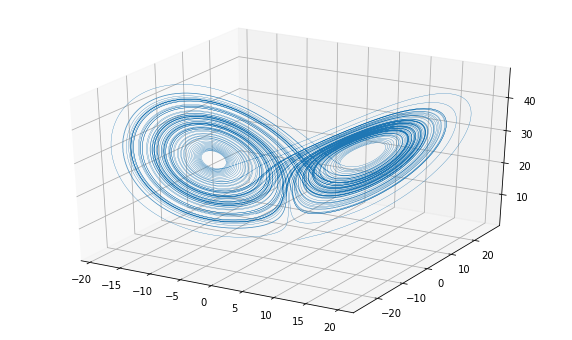
\includegraphics[width=0.7\linewidth]{chapter2/lorenzattractor}
	\caption[Three-dimensional plot of the Lorenz system.]{The Lorenz attractor in three dimensions with parameters $\sigma = 10$, $\beta = 8/3$, $\rho = 28$.}
	\label{fig:lorenzattractor}
\end{figure}

\begin{figure}[p]
	\centering
	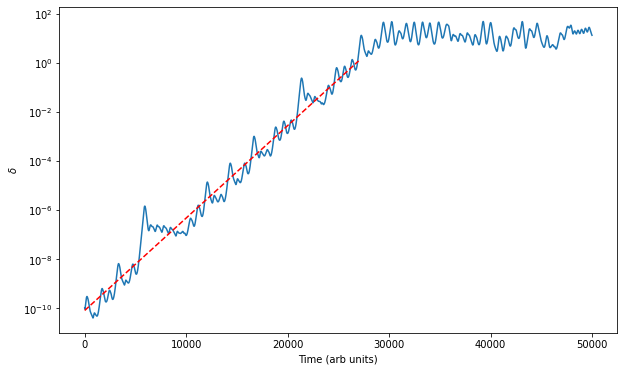
\includegraphics[width=0.7\linewidth]{chapter2/lorenzexp}
	\caption[Lyapunov exponent graphical approximation of the Lorenz system.]{The difference in trajectories through time of two nearby points, with an approximation of the MLE (dashed red). The plateau near the top is due to the maximal separation possible from the constraints of the system. }
	\label{fig:lorenzexp}
\end{figure}

\subsubsection{Lyapunov exponents in Hilbert space}
In order to find Lyapunov exponents in Hilbert space as required for quantum wavefunctions, we must devise a metric to find calculate distances. The norm of the wavefunctions is an obvious choice for this and has been used in prior works \cite{PhysRevA.83.043611}. This distance metric follows \begin{align}
	d^{(2)}(\psi_1, \psi_2; t) & = \frac{1}{2} \braket{\psi_1 - \psi_2}{\psi_1 - \psi_2} = \frac{1}{2} \int \dd{x} \abs{\psi_1(x, t) - \psi_2(x, t)}^2 \notag \\
		& = \int \dd{x} \left( \abs{\psi_1}^2 + \abs{\psi_2}^2 - 2 \psi_1^* \psi_2 \right). \label{eq:dist}
\end{align}
This metric will used in this paper to calculate distances between wavefunctions when determining the approximate maximal Lyapunov exponent. Note that as this is not a single trajectory and not in a phase space, this metric is an analogy to the maximal Lyapunov exponent. In the remainder of this work, we will refer to this metric as the Lyapunov exponent.


\section{Numerical methods}
%Numerical methods are procedures to solve a numerical problem, like finding solutions to a differential equation.
To see how the GPE evolves in time, the continuous spatial and time components must first be split into many smaller discrete slices---this is known as \textit{discretization}. Discretization has an innate error, growing for every increase in slice size. This error can be reduced by choosing minimized spatial and time deltas that adequately fit the problem, a trade-off with requiring excessive computational resources.

In this paper, we will use Runge-Kutta (RK) methods for approximating solutions of the GPE by solving the differential equation in time. To use this method, the spatial component must first be discretized using matrices described in Chapter 3. We will use the \texttt{solve\_ivp} function provided by SciPy as an implementation of the explicit Runge-Kutta method of order 5. This function has controllable tolerances, allowing an estimation of an error due to temporal discretization. 
\addchapheadtotoc

\chapter{Procedures}

The Gross-Pitaevskii equation is simulated using Python using a spatial finite difference method and the Runge-Kutta method for the time evolution. Numpy is used to discretize the wavefunction with matrices and the SciPy package is used to evolve the wavefunction through time. An initial wavefunction generated as a sinusoid independent of the lattice size and evolved prior to perturbation. This wavefunction is perturbed by superimposing a small sinusoid and both functions are allowed to evolve independently. The difference of these wavefunctions is recorded and a Lyapunov exponent can be calculated. 

\section{Numerical Derivatives}
For the spatial discretization, a 2D diagonal matrix was used to calculate the first derivative. To begin, recall the definition of a derivative, \begin{equation}
	f'(x) = \lim_{h \to 0} \frac{ f(x+h) - f(x) }{h} + O(h).
\end{equation}
To approximate the limit, we can take $h$ to be a small finite value relative to the target function $f(x)$. This equation is known as the \textit{forward difference}, as $h$ is \textit{forward} of $x$. In a similar fashion, the backward difference is given as \begin{equation}
	f'(x) = \lim_{h \to 0} \frac{f(x-h) - f(x)}{h} + O(h).
\end{equation}
Both the forward and backward differences can be averaged for a more accurate central difference approximation, \begin{equation}
	f'(x) = \lim_{h \to 0} \frac{f\left(x+\frac{h}{2}\right) - f\left(x - \frac{h}{2}\right)}{h} + O(h^2).
\end{equation}
For the second-order central difference approximation, it can be shown either directly or through the Taylor expansion \begin{equation}
	f''(x) = \lim_{h \to 0} \frac{f(x+h) - 2f(x) + f(x-h)}{h^2} + O(h^3).
\end{equation}
Note that this method has some truncation error due to the Taylor expansion. Additional higher-order terms $O(h^3)$ can be added for better precision at the expense of computational cost. 

\subsection{Matrix formulation}
In the second-order central difference approximation, each term at point $x$ depends on the previous and next spatial term. As the derivative operator is linear and many Python libraries support matrices including NumPy, we can convert the second-order derivative operator to a matrix. For a given function $f(x)$ discretized over $x$, the second derivative can be calculated using the matrices, \begin{align}
		\ket{f''(x)} & = \hat{D} \ket{f(x)} \notag \\
		\begin{pmatrix}
			f''(x_0) \\
			f''(x_1) \\
			f''(x_2) \\
			\vdots \\
			f''(x_{N-1})
		\end{pmatrix} & = \frac{1}{h^2}\begin{pmatrix}
			-2 & 1 & \\
			1 & -2 & 1 \\
			  & 1 & -2 & 1 \\
			  & & \ddots & \ddots & \ddots \\
			  & & & 1 & -2 & 1
	\end{pmatrix} \begin{pmatrix}
		f(x_0) \\
		f(x_1) \\
		f(x_2) \\
		\vdots \\
		f(x_{N-1})
	\end{pmatrix} \label{eq:mtxd2}.
	\end{align}
	For periodic boundary conditions, the first term of the derivative must wrap around and use the last term in the derivative calculation, and vice versa. This results in modifying \eqref{eq:mtxd2} to  \begin{align}
		\begin{pmatrix}
			f''(x_0) \\
			f''(x_1) \\
			f''(x_2) \\
			\vdots \\
			f''(x_{N-1})
		\end{pmatrix} & = \frac{1}{h^2}\begin{pmatrix}
			-2 & 1 & & & & 1\\
			1 & -2 & 1 \\
			& 1 & -2 & 1 \\
			& & \ddots & \ddots & \ddots \\
			1 & & & 1 & -2 & 1
		\end{pmatrix} \begin{pmatrix}
			f(x_0) \\
			f(x_1) \\
			f(x_2) \\
			\vdots \\
			f(x_{N-1})
		\end{pmatrix} \label{eq:mtxd2_periodic}.
	\end{align}
	From this matrix, the one-dimensional Laplacian term in the Gross-Pitaevskii equation can be approximated.
	
	\section{Gross-Pitaevskii equation and time evolution}
	From the second derivative matrix \eqref{eq:mtxd2_periodic}, the Python function in Listing \ref{lst:gpe} can be used to evolve the time-dependent Gross-Pitaevskii equation over time with \texttt{solve\_ivp} from the SciPy package. This function solves \eqref{eq:gpe} for $\pdv{\Psi}{t}$. Using this function definition, the Runge-Kutta method can be applied as an adaptive solver and the time evolution can be observed, resulting in a 2D matrix over time and space. Additionally, the relative and absolute tolerances can be lowered in the solver to ensure high precision.

	\begin{figure}[h]
		\begin{lstlisting}[language=Python, caption={The \texttt{solve\_ivp} wrapper function for the Gross-Pitaevskii equation. This function approximates \eqref{eq:gpe}.}, label={lst:gpe}]
	def compute_dpsi_dt(t, psi):
		""" Return dpsi/dt for the GPE. """
		phase = 1 / (1j * hbar * cooling_phase / np.abs(cooling_phase))
		n = abs(psi)**2
		return phase * (-hbar / 2 / m * (D2 @ psi) + (V(x) + g * n) * psi)
		\end{lstlisting}
	\end{figure}

	\section{Initial many-body wavefunction}
	Before perturbing the wavefunction when calculating the Lyapunov exponent, an initial wavefunction must be generated. Here, a function was used to generate sinusoidal noise with perioidic boundary conditions. This function generates an initial state independent of the dimensions of the lattice spacing. This function is shown in Listing \ref{lst:fouriernoise}.

	\section{Lyapunov exponent calculation}
	To calculate the Lyapunov exponent of the Gross-Pitaevskii equation, first we must generate a wavefunction and a perturbed copy, then evolve both through time and calculate the difference in Hilbert space. The Lyapunov exponent must be approximated, as the limits are not feasible as the time and spatial components are finite and discrete. Here, we will use an analog to the Lyapunov exponent by evolving the system until the distance is maximized and plateaued, as shown in Figure \ref{fig:lorenzexp}.
	
	An initial wavefunction is generated using Listing \ref{lst:fouriernoise}. A perturbed wavefunction is created by superimposing a small-amplitude sinusoid on the initial function. Both functions are evolved independently and the difference in wavefunctions are calculated over time using \eqref{eq:dist}. After a set time, the perturbed wavefunction is ``pulled back'' so the two wavefunctions meet, shown in Figure \ref{fig:pullbacks}. This process is repeated several times to ensure a maximal exponent can be found. The Lyapunov exponent is calculated for each iteration by taking a exponential fit of the differences as a function of time in the direction of the maximal Lyapunov exponent. 


	\begin{figure}[p]
		\centering
		 \begin{subfigure}[b]{0.75\textwidth}
			\centering
			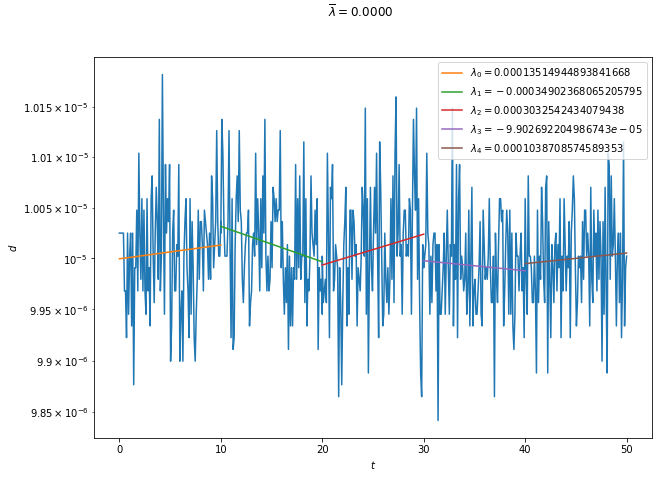
\includegraphics[width=\linewidth]{chapter3/pullbacks0}
			\caption{$g=0$}
			\label{fig:pullbacks0}
		\end{subfigure}
		
			\vspace{2em}
			
		 \begin{subfigure}[b]{0.75\textwidth}
			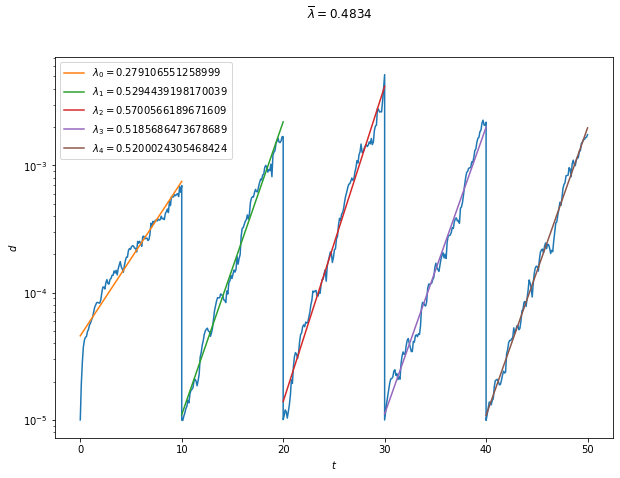
\includegraphics[width=\linewidth]{chapter3/pullbacks}
			\caption{$g=10$}
		\end{subfigure}
		\caption[An example of pulling back the perturbed wavefunction.]{An example of pulling back the perturbed wavefunction for two cases: the normal Schr\"odinger equation and the nonlinear case. }
		\label{fig:pullbacks}
	\end{figure}
	

	To ensure numerical error is minimized, after evolving the wavefunction through time, the wavefunction is evolved backwards through time. The difference between the original wavefunction and the reverse-time-evolved function must be within a small tolerance to ensure accuracy.
	
	Additionally, for the $g=0$ case, the Gross-Pitaevskii equation is the regular Schr\"odinger equation. This case is linear and should give no chaotic motion, and we should expect a zero Lyapunov exponent.
	
	\section{Experimental values}
	In the simulation, we set $\hbar=1$ and mass $m=1$. The periodic lattice is set to a length of $L=10$ length units, divided into 400 segments. The maximum time step size is set to $\Delta t = 0.01$ time units in the RK45 solver.	The units of time are \begin{align*}
		[t] & = \frac{[L]^2}{10^2} \frac{[m]}{[\hbar]}.
		\end{align*}
	The perturbation amplitude is set to \num{e-5} length units. When varying $g$, the system is allowed to evolve for 1 time unit with 100 steps. This process is repeated 5 times per $g$ value.
%	TODO: write out the units. 
%	
%	the time unit can be determined with \begin{align*}
%			t & = m L^2 / \hbar?
%		\end{align*}
%	How to go about finding what the time units are in SI units?
%	
%	Units of $g$?
	
\addchapheadtotoc

\chapter{Findings}
The Gross-Pitaevskii equation exhibits numerical chaos when an initial turbulent state evolves in zero potential. Chaos is seen for positive values of $g$. For positive nonlinear coupling constant $g$, the relationship between the Lyapunov exponent is seemingly linear, as shown in Figure \ref{fig:glam}. For negative $g$, there is no clear relationship. Shown in Figure \ref{fig:gline}, applying a linear regression for positive $g$ results in \begin{equation}
	\lambda(g) = \num{0.04996 \pm 0.00206} g + \num{0.0197 \pm 0.0125},
\end{equation}
with $p<0.01$ and $R^2=0.986$, indicating correlation and a high degree of fitment. 
\begin{figure}[p]
	\centering
	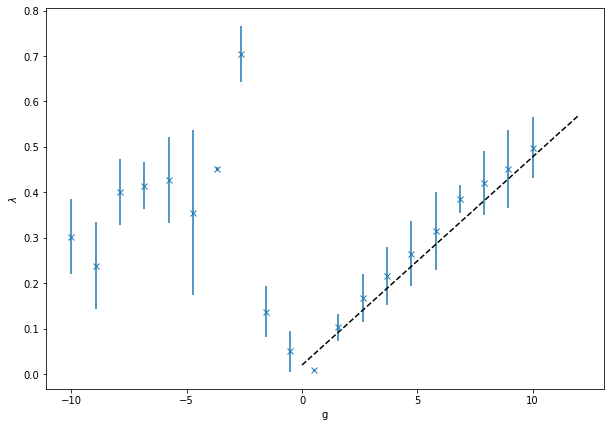
\includegraphics[width=0.7\linewidth]{chapter4/g_lam}
	\caption{The effect of $g$ on the Lyapunov exponent. Note the cross represents the mean for that sample and the error bars denote the standard deviation from $N=5$ samples.}
	\label{fig:glam}
\end{figure}

\begin{figure}[p]
	\centering
	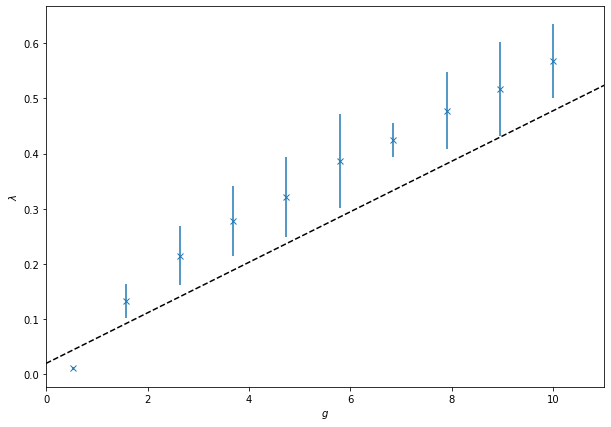
\includegraphics[width=0.7\linewidth]{chapter4/g_line}
	\caption{Linear fit on positive coupling constant $g$ versus the Lyapunov exponent.}
	\label{fig:gline}
\end{figure}



\section{Error analysis}
Several steps were taken to ensure error is minimized. First, both wavefunctions are evolved backward in time to ensure convergence to their original wavefunction. Next, we check the role of tolerances used in the solver and its effect on the Lyapunov exponent. Lastly, the role of machine precision is discussed.


\subsection{Reverse time evolution}
After each experiment, the wavefunctions are evolved backwards in time to the original time step, attempting to perfectly recover the original wavefunction, akin to the Loschmidt echo. This wavefunction is compared to the original wavefunction to ensure error in the solver is minimized by iterating over the spatial dimension and finding the difference at each point. The time-reversed wavefunction were found to be equal to the original within an absolute tolerance of \num{1e-10}. This value is beyond the tolerances of the solver, indicating recovery of the original wavefunction.


\subsubsection{Role of solver tolerances}
The Gross-Pitaevskii equation with coupling constant $g=0$ returns the Schr\"odinger equation, a linear differential equation and we should expect a Lyapunov exponent of zero. Experimentally, the Lyapunov exponent for this case was found to be zero for high-precision absolute and relative solver tolerances of \num{1e-10} and smaller. For lower-precision tolerances, the solver fails, as shown in Figure \ref{fig:tollam}. For the nonzero $g$, a solver tolerance of \num{1e-10} is then specified.

\begin{figure}[p]
	\centering
	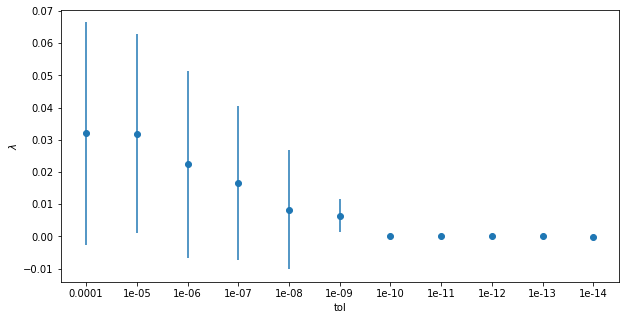
\includegraphics[width=\linewidth]{chapter4/tol_lam}
	\caption{Effect of solver tolerances on the Lyapunov exponent for the non-chaotic Schr\"odinger equation. The Lyapunov exponent is expected to return zero. For higher tolerances ($<\num{1e-10}$), the error is significantly increased indicating poor precision and solver failure.}
	\label{fig:tollam}
\end{figure}

\subsubsection{Role of machine precision and spatial derivative error}
In the simulation, NumPy is a library used for performing mathematical and matrix operations. The library relies on 64-bit floating point numbers, as specified by IEEE-754. The machine precision of floating point numbers as defined in IEEE-754 is the limiting precision on floating point numbers in the simulated Gross-Pitaevskii equation \cite{1985--ieee754}. This value is defined in the specification as \begin{equation}
	\epsilon = \num{2.22e-16}.
\end{equation}
This value must be taken into account when setting both the lattice spacing $h$ and the solver tolerances.
\addchapheadtotoc

\chapter{Conclusions}
We confirm our hypothesis that the nonlinearity of the one-dimensional Gross-Pitaevskii equation gives rise to chaos.
We have seen for positive $g$ returns positive Lyapunov exponents, implying chaotic motion in Bose-Einstein condensates. For the $g=0$ case, our assumption is correct in that it returns a zero Lyapunov exponent, which is consistent with the linearity of the Schr\"odinger equation. For positive coupling constant $g$, there is a proportionality found between the constant and the Lyapunov exponent. The nonlinear coupling constant term is seemingly the cause of this chaos, understandably as chaos cannot arise from linearity. The chaotic dependence on $g$ reproduces the results by Brezinova, et al. \cite{PhysRevA.83.043611} using finite difference numerical methods. It is still unclear whether this chaos is caused by the failure of the GPE or of it exists in reality.

When finding the Lyapunov exponent, it was noted that the first iteration before pulling back was likely in the wrong direction of the maximal Lyapunov exponent. This Lyapunov exponent should be dropped or additional, perhaps hundreds, iterations should be run. Additional research is necessary to extend these findings to higher dimensions and to systems with quantum turbulence.
\appendix

%%%%%%%%%% DON'T DELETE THIS, REVERTS NUMBERING BACK %%%%%%%%%%%%%
\makeatletter
\renewcommand{\@makechapterhead}[1]{\vspace *{-10\p@ }{\parindent \z@ 
\raggedright \normalfont \ifnum \c@secnumdepth >\m@ne \Huge \bfseries 
\@chapapp \space \thechapter \vskip 10\p@ \fi #1\par \nobreak \vskip 30\p@ }}
\makeatother
%%%%%%%%%% DON'T DELETE THIS, REVERTS NUMBERING BACK %%%%%%%%%%%%%





% Bibliography
\begingroup
    \setlength\bibitemsep{10pt}
    \linespread{1}\selectfont
    \printbibliography[title=REFERENCES]
\endgroup
\addcontentsline{toc}{part}{REFERENCES}

% Appendices
% \appendix

%%%%%%%%%% DON'T DELETE THIS, REVERTS NUMBERING BACK %%%%%%%%%%%%%
\makeatletter
\renewcommand{\@makechapterhead}[1]{\vspace *{-10\p@ }{\parindent \z@ 
\raggedright \normalfont \ifnum \c@secnumdepth >\m@ne \Huge \bfseries 
\@chapapp \space \thechapter \vskip 10\p@ \fi #1\par \nobreak \vskip 30\p@ }}
\makeatother
%%%%%%%%%% DON'T DELETE THIS, REVERTS NUMBERING BACK %%%%%%%%%%%%%





\end{document}
